\chapter{Application to the kink instability}
\label{chp:kink_instability}

\graphicspath{{images/kink_instability/}}

\section{Introduction}
\label{sec:kink_introduction}

In this chapter I investigate the effects of anisotropic viscosity on the kink instability~\cite{hoodKinkInstabilitySolar1979, hoodCoronalHeatingMagnetic2009}, believed to be a trigger for flares~\cite{srivastavaObservationKinkInstability2010} and an important mechanism in the theory of coronal heating through nanoflares~\cite{browningHeatingCoronaNanoflares2008a}. The instability has also been studied using shock viscosity~\cite{hoodCoronalHeatingMagnetic2009,barefordShockHeatingNumerical2015} but a detailed investigation of the effects of Newtonian and Braginskii viscosity has not, to the best of my knowledge, been performed. In particular, the main aim of this investigation is to provide insight into the effect of the choice of viscosity model on the nonlinear dynamics and relaxation of a twisted coronal loop, where the kink instability converts magnetic energy to heat through Ohmic heating generated via current structures and through viscous heating generated via flow structures. I aim to give an estimate of how well viscous heating (using both isotropic and anisotropic models) performs when compared with Ohmic heating. This study extends previous work~\cite{hoodCoronalHeatingMagnetic2009} which also considers the kink instability in a zero-current loop (details given below). However, in contrast to~\cite{hoodCoronalHeatingMagnetic2009}, only background resistivity and viscosity are used as the two mechanisms of heat generation (that is, shock viscosity and anomalous resistivity are disabled). This investigation also provides further validation of the switching model in a simpler topology to that used by MacTaggart et al.~\cite{mactaggartBraginskiiMagnetohydrodynamicsArbitrary2017}, simpler in that there are no null points present in the field at any time.

The layout of the chapter is as follows. The coronal loop model is described in Section~\ref{sec:model-setup}. Details of the numerical setup and methods used in the analysis of the simulation results are presented in Section~\ref{sec:general-numerical-setup}. Detailed numerical results of a typical case of a kink instability are given in Section~\ref{sec:results} with a particular focus on how the different viscosity models affect its nonlinear evolution. The results of the typical case are confirmed and generalised by a parameter study in Section~\ref{sec:results2} where the dependences of the Ohmic and the viscous heating on the resistivity and the dynamic viscosity are explored. Conclusions are summarised in Section~\ref{sec:conclusions}.

This chapter is an adaptation of a previously published paper~\cite{quinnEffectAnisotropicViscosity2020a}. 

\section{Coronal loop model}
\label{sec:model-setup}

A twisted magnetic flux rope is used as the model of an idealised coronal loop. The domain is a Cartesian box of dimension $[-2\text{ Mm},2\text{ Mm}] \times [-2\text{ Mm},2\text{ Mm}] \times [-10\text{ Mm},10\text{ Mm}]$ in the $x$, $y$ and $z$-directions, respectively. The state of the plasma is typical of the corona, with density $\rho$ initially $1.67\times 10^{-12} \text{ kg m}^{-3}$, and with plasma pressure $p$ such that the temperature of the plasma $T$ is initially $2\times10^{4} \text{ K}$ everywhere in the domain. The magnetic field $\vec{B}$ is constructed so that it is initially force-free and with zero axial current, line-tied at the boundaries, and twisted such that it is linearly unstable to the ideal kink instability. This configuration allows direct comparison to previous studies that use similar magnetic field configurations~\cite{hoodCoronalHeatingMagnetic2009,barefordShockHeatingNumerical2015,bothaObservationalSignaturesCoronal2012}. The field outside the flux tube is straight and has a strength of $5\times10^{-3} \text{ T}$. Given this temperature and magnetic field strength, the plasma beta is initially $\beta \approx 10^{-5}$, a value realistic for the corona. The evolution of this flux tube is governed by the nonlinear MHD equations described in section~\ref{sec:mhd_equations}.

\begin{table}[t]
\centering
\begin{tabular}{ccc|ccc}
$B_0$ & $L_0$ & $\rho_0$ & $u_A = B_0 / \sqrt{\rho_0 \mu_0}$ & $t_A = L_0/u_A$ & $T_0$ \\ \midrule
$5 \times 10^{-3} \ \text{T}$ & $1\ \text{Mm}$ & $1.67 \times 10^{-12} \ \text{kgm}^{-3}$ & $3.45\ \text{Mms}^{-1}$ & $0.29\ \text{s}$ & $1.73 \times 10^{9}K$\\
\end{tabular}
\caption{Reference values for the magnetic field, length, density, and
  temperature. These are used to non-dimensionalise the MHD
  equations \eqref{eq:mhda}--\eqref{eq:energy} and to calculate the reference values for velocity, time and temperature.}
\label{tab:reference-values}
\end{table}

The magnetic field is considered force-free, that is the field is constructed such that the Lorentz force is zero, or $(\nabla \times \vec{B})\times \vec{B} = 0$. In cylindrical coordinates $(r,\theta,z)$, the chosen force-free magnetic field takes the form $\nabla \times \vec{B} = \alpha(r)\vec{B}$, where $\alpha(r)$ is a function of a particular form that ensures the total axial current is zero. Aligning with previous work by Hood et al.~\cite{hoodCoronalHeatingMagnetic2009}, the smooth $\alpha(r)$ profile given as Case 3 in~\cite{hoodCoronalHeatingMagnetic2009} is used. Using this profile, the equilibrium magnetic field $\vec{B}$ is written as 
\begin{equation}
\begin{aligned}
  \label{eq:field-profile-r-lt-1}
  B_{\theta} &= \lambda r {(1 - r^2)}^3,\\
  B_z &= \sqrt{1 - \frac{\lambda^2}{7} + \frac{\lambda^2}{7}{(1 - r^2)}^7 - \lambda^2 r^2 {(1-r^2)}^6},\\
  \alpha(r) &= \frac{2 \lambda {(1-r^2)}^2 {(1-4r^2)}}{B_z},
\end{aligned}
\end{equation}
for $r \leq 1$ and
\begin{equation}
\begin{aligned}
  \label{eq:field-profile-r-gt-1}
  B_{\theta} &= 0 \\
  B_z &= \sqrt{1 - \frac{\lambda^2}{7}}\\
  \alpha(r) &= 0 ,
\end{aligned}
\end{equation}
for $r > 1$, where $\lambda$ is a parameter measuring the twist in the tube. The radial field throughout the domain is set to $B_r = 0$. As is done in~\cite{hoodCoronalHeatingMagnetic2009}, $\lambda = 1.8$ to ensure the tube is unstable to the ideal kink instability. The equilibrium velocity for this magnetic field configuration is $\vec{u} = \vec{0}$.

\begin{figure}[t]
  \centering
  \begin{subfigure}[b]{0.48\textwidth}
  \begin{center}
    \begin{overpic}[width=\textwidth]{field_line_plots/cropped/v1e-4r5e-4.5-isotropic_0000_cropped.png}
      \put (50,5) {\small\textbf{(a)}}
    \end{overpic}
  \end{center}
  \end{subfigure}
  \begin{subfigure}[b]{0.48\textwidth}
  \begin{center}
    \begin{overpic}[width=\textwidth]{alpha_profile.pdf}
      \put (47,54) {\small\textbf{(b)}}
    \end{overpic}
  \end{center}
  \end{subfigure}
  \caption{\textit{The initial field configuration.} In \textbf{(a)} field lines are plotted corresponding to inner (red), outer (blue) and straight (yellow) regions of twist, with slices of $\alpha(r)$ shown at the footpoints. In the slices, red corresponds to $\alpha(r) > 0$, blue to $\alpha(r) < 0$ and white to $\alpha(r) = 0$. In \textbf{(b)} the profiles of $\alpha(r)$ and the field components $B_z$ and $B_{\theta}$ across the flux tube are plotted.}
\label{fig:field_configuration}
\end{figure}

The form of $\alpha(r)$ in equations~\eqref{eq:field-profile-r-lt-1} and~\eqref{eq:field-profile-r-gt-1} splits the profile of the flux tube into three twist regions, the inner region of positive twist ($r\le0.5$), the outer region of negative twist ($0.5<r<1$) and the straight-field region of zero twist ($r\ge1$) as shown in Figures~\ref{fig:field_configuration}(a) and (b). These figures also illustrate the equilibrium field. Since the inner region is more tightly twisted, this field configuration results in only the inner region becoming unstable to the kink instability, rather than the global instability seen in non-zero-current loops~\cite{hoodKinkInstabilitySolar1979}. The regions of twist are used later to define a measure of reconnection.

Although the initial temperature is prescribed as $T=2\times10^{4} \text{ K}$, the equations simulated by the code are written using internal energy, thus the temperature is converted to internal energy using the non-dimensional relation $\varepsilon = T/(1-\gamma)$. Hence, the initial non-dimensionalised density and internal energy are uniformly given by
\begin{equation}
  \rho = 1,\quad \varepsilon = 8.66 \times 10^{-4},
\end{equation}
and have been non-dimensionalised using the reference values found in Table~\ref{tab:reference-values}. The initial magnetic field and velocity are set to their equilibrium states, discussed above, with the addition of a small perturbation.

In order to make a meaningful comparison of the following results with those of~\cite{hoodCoronalHeatingMagnetic2009}, identical initial magnetic field and velocity perturbations are used, calculated via a linear stability analysis (in ideal MHD) applied to a similar flux tube that uses a constant, piecewise profile for $\alpha(r)$~\cite{vanderlindenCompleteCoronalLoop1999,browningSolarCoronalHeating2003c,browningHeatingCoronaNanoflares2008a}.

At the boundaries, the line-tied condition on the magnetic field is satisfied by ensuring the field is constant and equal to its initial values given by equations~\eqref{eq:field-profile-r-lt-1} and~\eqref{eq:field-profile-r-gt-1}. Similarly, on the boundaries the density, internal energy and velocity $\vec{u}$ are considered constant and equal to their initial values. To close the system, the fluxes of all variables through each of the boundaries are set to zero. That is, on the $x$-boundary,
\begin{equation}
  \frac{\partial \vec{B}}{\partial x} = \frac{\partial \vec{u}}{\partial x} = \vec{0}; \quad \frac{\partial \rho}{\partial x} = \frac{\partial \varepsilon}{\partial x} = 0 \quad \text{for } x=\pm 2,
\end{equation}
and similarly, the $y$ and $z$ derivatives are zero on the $y=\pm2$ and $z=\pm10$ boundaries, respectively.

Since there are no nulls created during the evolution of the kink instability, the field remains strong everywhere and the viscosity reverts to fully parallel. To ensure this, the switching model~\ref{eq:switching_model} is used with the von Mises switching function~\ref{eq:switching_function} where $a_0 = 150$. 

\section{Methods}
\label{sec:general-numerical-setup}

In this section the parameters of the numerical setup is presented, and various tools and quantities used in the proceeding analysis are described.

\subsection{Numerical setup}

The MHD equations~\eqref{eq:mhda}---\eqref{eq:energy} were solved numerically using the Lare3d code~\cite{arberStaggeredGridLagrangian2001}, previously described in chapter~\ref{chp:numerical_methods}. Shock viscosity was disabled in order to properly investigate the effect of different viscosity models. In order to compare results with those of Hood et al.~\cite{hoodCoronalHeatingMagnetic2009} numerical tests were performed using shock viscosity instead of either the switching or isotropic models. Using the default shock viscosity parameters present in the code, the behaviour closely mirrors that of isotropic viscosity with $\nu\approx 5\times10^{-4}$. When both switching and shock viscosity are enabled, the shock viscosity dominates and, again, the behaviour mirrors that of isotropic viscosity.

The simulations were run at a resolution of $350 \times 350 \times 700$, with the exception of the parameter studies, which were run at a slightly higher resolution of $400 \times 400 \times 800$. Since the switching viscosity only acts parallel to the magnetic field, in perpendicular directions numerical diffusion dominates. By running several simulations at resolutions of $250 \times 250 \times 500$ up to $500 \times 500 \times 1000$, it was found that the effect of resolution was negligibly small until around $t=150$, well after the nonlinear phase of the instability. After this time there were some quantitative differences in outputs for different resolutions. However, the qualitative behaviour, described later, does not strongly depend on the resolution.

The numerical diffusion present in the simulations (due to the finite difference scheme employed in Lare3d) is estimated as $\tilde{\nu} = \tilde{\eta} = \tilde{u}_x L_x/N_x^2$. Taking a typical velocity of $\tilde{u}_x = 1$, i.e.\ the Alfv\'en velocity; $N_x = 350$ as the number of grid-points in the $x$-direction; and $L_x = 4$ as the length in the $x$ direction, the numerical diffusion coefficient is estimated as $\tilde{\nu} = \tilde{\eta} \approx 10^{-5}$. This provides a theoretical lower bound on simulating a physical viscosity or resistivity. In practice, setting the physical resistivity lower than $\eta \approx 5\times10^{-5}$ results in behaviour that does not converge with increasing resolution. This gives a practical lower bound for diffusion coefficients of $\tilde{\nu} = \tilde{\eta} \approx 5 \times 10^{-5}$. Thus, all results presented use physical diffusion coefficients (either viscosity or resistivity) greater than this lower bound.

\subsection{Methods of analysis}

\subsubsection{Connectivity}

The mean change in field line connectivity $\Delta\Phi_c$ is used as a practical measure of reconnection rate. The connectivity of a given field line $\Phi_c$ is determined by comparing its start and end points. Any field line that begins at one location in one of the loop footpoints will map to a corresponding point in the opposite footpoint. Following field lines from their starting point at $z=-10$ to their end point at $z=10$, lines are labelled depending on the twist regions in which they start and end. Initially, the field lines within each distinct region map one-to-one to the same region. As the field reconnects radially during the instability, field lines begin to start and end in different twist zones. The rate of reconnection is estimated by tracking the number of field lines that have changed twist zones within a set time period. This also serves as a visual representation of where such reconnection is occurring. It should be noted that this measure of reconnection does not take into account azimuthal reconnection (that is reconnection within the same twist zone). As such, it is only a partial measure of reconnection.

In practice, magnetic field output is saved from the code at intervals of $\Delta t = 5$. The visualisation tool Mayavi~\cite{ramachandran2011mayavi} is used to compute the magnetic field lines over a grid of starting points $(x_i, y_j)$ at a given time $n \Delta t$, where $n$ indexes the output files. This process gives a connectivity map $\Phi_c^{(n)}(x_i, y_j)$ across the profile of the flux tube. The mean difference in connectivity $\Delta \Phi_c^{(n)}$ at time $n\Delta t$ is found by subtracting one connectivity map from the previous and then taking the mean across all points $(x_i, y_j)$,
\begin{equation}
  \Delta \Phi_c^{(n)} = \frac{1}{N_x N_y} \sum_{i=1}^{N_x} \sum_{j=1}^{N_y} (\Phi_c^{(n)}(x_i, y_j) - \Phi_c^{(n-1)}(x_i, y_j)).
\end{equation}

\subsubsection{Parallel electric field}

Another useful measure of magnetic reconnection is the maximum value of the integral of the electric field parallel to the magnetic field $E_{\parallel} = \eta {(\vec{\jmath} \cdot \vec{B})}/|\vec{B}|$ along a magnetic field line~\cite{galsgaardSteadyStateReconnection2011,priestNatureThreedimensionalMagnetic2003,schindlerGeneralMagneticReconnection1988},
\begin{equation}
  \Phi = \int_{C} \eta \frac{(\vec{\jmath} \cdot \vec{B})}{|\vec{B}|}\ {\rm d}l,
\end{equation}
where $C$ is a magnetic field line with start and end points within the footpoints at $z\pm10$.

Using a similar method as in the calculation of connectivity, Mayavi is employed to compute magnetic field lines using a grid of field line starting points $(x_i, y_j)$ at a given time. The local value of the modulus of the parallel electric field, $|E_{\parallel}| = |\eta \vec{\jmath} \cdot \vec{B}|$, is summed along each of the magnetic field lines to give a distribution $\Phi(x_i, y_j)$ across the profile of the field. The maximum of this distribution gives a measure of the reconnection rate.

It can be argued that the reconnection rate calculated by taking the global maximum is only the rate for one region of magnetic diffusion, and the nonlinear phase of the kink instability creates multiple diffusion regions in its development. One way to calculate the reconnection rate for each region is via the algorithm described in~\cite{pontinDynamicsBraidedCoronal2011}, which dissects the distribution $\Phi(x_i, y_j)$ into separate regions before finding the maxima corresponding to the reconnection rate per diffusion region. In practice, the current structures created by the kink instability in the reported results are simple enough that this extended analysis is unnecessary.

\subsubsection{Other observables}

In the course of analysing the simulation outputs, use is also made of the volume-integrated parallel and perpendicular kinetic energies,
\begin{equation}
  \label{eq:kinetic_energies}
  \text{KE}_{\parallel} = \frac{1}{2} \int_V \rho\frac{(\vec{u}\cdot\vec{B})^2}{|\vec{B}|^2}\ \text{d}V; \quad
  \text{KE}_{\perp} = \frac{1}{2} \int_V \rho|\vec{u}|^2\ \text{d}V - \text{KE}_{\parallel},
\end{equation}
the magnetic energy,
\begin{equation}
  \label{eq:magnetic_energy}
   \text{ME} = \frac12\int_V |\vec{B}|^2\ \text{d}V,
\end{equation}
and the total Ohmic heating generated by time $T$,
\begin{equation}
  \label{eq:ohmic_heating}
  Q_{\eta} = \eta \int_0^{T} \int_V |\vec{\jmath}|^2\ \text{d}V \text{d}t.
\end{equation}
The time and volume-integrated viscous heating rate can be written
in the form
\begin{equation}
  \label{eq:iso_viscous_heating}
  Q_{\nu}^{iso} = \frac{\nu}{2} \int_0^T \int_V
  \text{tr}(\ten{W}^2)\  \text{d}V \text{d}t,
\end{equation}
for the isotropic viscous stress
tensor~\eqref{eq:isotropic_viscous_tensor} and in the form
\begin{equation}
  \label{eq:aniso_viscous_heating}
  Q_{\nu}^{aniso} = \nu \int_0^T \int_V \left[ (1-s^2(|\vec{B}|)\frac{1}{2}\text{tr}(\ten{W}^2) + s^2(|\vec{B}|)\frac{3 }{4} ((\ten{W} \vec{b}) \cdot \vec{b})^2\ \right] \text{d}V \text{d}t,
\end{equation}
for the switching viscous stress tensor~\eqref{eq:switching_model} using the von Mises switching function, respectively.

\section{Nonlinear evolution of a typical case}
\label{sec:results}

In this section, I present results from a pair of simulations with a single choice of viscosity and resistivity. This provides an opportunity to analyse, in detail, the onset and evolution of the kink instability in a single, typical case, in particular comparing the effect of the two viscosity models. Parameter studies illustrating that the observed dynamics are typical are presented in Section~\ref{sec:results2}. The pair of simulations differ only in that isotropic viscosity is used in one case and switching viscosity is used in the other. The diffusion parameters used in both simulations are $\nu = 10^{-4},\ \eta = 5\times 10^{-4.5}$, both small but suitably above the threshold of numerical diffusion discussed in Section~\ref{sec:general-numerical-setup}. The chosen value of $\nu$ is within the range of typical values found in the real corona, that is between $10^{-8}$ and $10^{-3}$~\cite{rudermanSlowSurfaceWave2000a}. All other parameters are identical in both cases and are kept fixed to the values specified in Section~\ref{sec:general-numerical-setup}. Due to the strength of the field and lack of null points, it is measured that $s=1$ throughout the entire domain, thus the switching model reverts to the strong field approximation of the Braginskii tensor~\eqref{eq:braginskii_parallel_term}.

\subsection{Linear phase}

\begin{figure}[t]
  \centering
  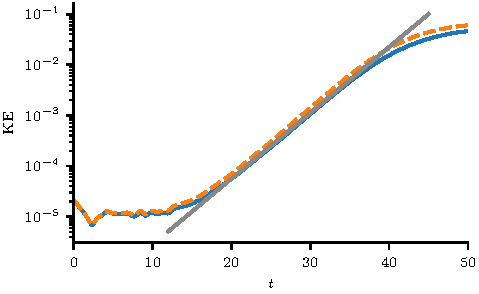
\includegraphics[width=0.5\linewidth]{log_kinetic_energy_over_time.pdf}
  \caption{\textit{Logarithmic plot of the total kinetic
      energy during the linear phase.} Overlaid is a straight
    line corresponding to the linear growth rate $\sigma = 0.13$. The
    isotropic case is represented as a blue, solid line and the
    switching case as an orange, dashed line. Though the kinetic energy is initially slightly greater using the switching model, the growth rate appears unaffected by choice of viscosity model. The duration of the linear phase also appears to be negligibly affected.}%
  \label{fig:log_kinetic_energy_over_time}
\end{figure}

The linear development of the kink instability lasts until $t\approx 35$ as illustrated in   Figure~\ref{fig:log_kinetic_energy_over_time} and has a measured linear growth rate of $\sigma = 0.13$. Since the initial velocity perturbation is calculated from an ideal and inviscid MHD model with a piecewise constant $\alpha(r)$ in the equilibrium configuration, the perturbation does not necessarily represent the most unstable mode for the setup of the simulation. For this reason there is a brief transient period before the exponential rise of the instability at $t\approx10$, as shown in Figure~\ref{fig:log_kinetic_energy_over_time}. The isotropic model damps this initial velocity perturbation more than the switching model, leading to a small difference in kinetic energy during the growth of the linear instability, although the growth rate appears to be identical across the two models. The duration of the linear phase is also unaffected by the choice of viscosity model.

\begin{figure}[t]
  \centering
    \begin{subfigure}{0.49\textwidth}
      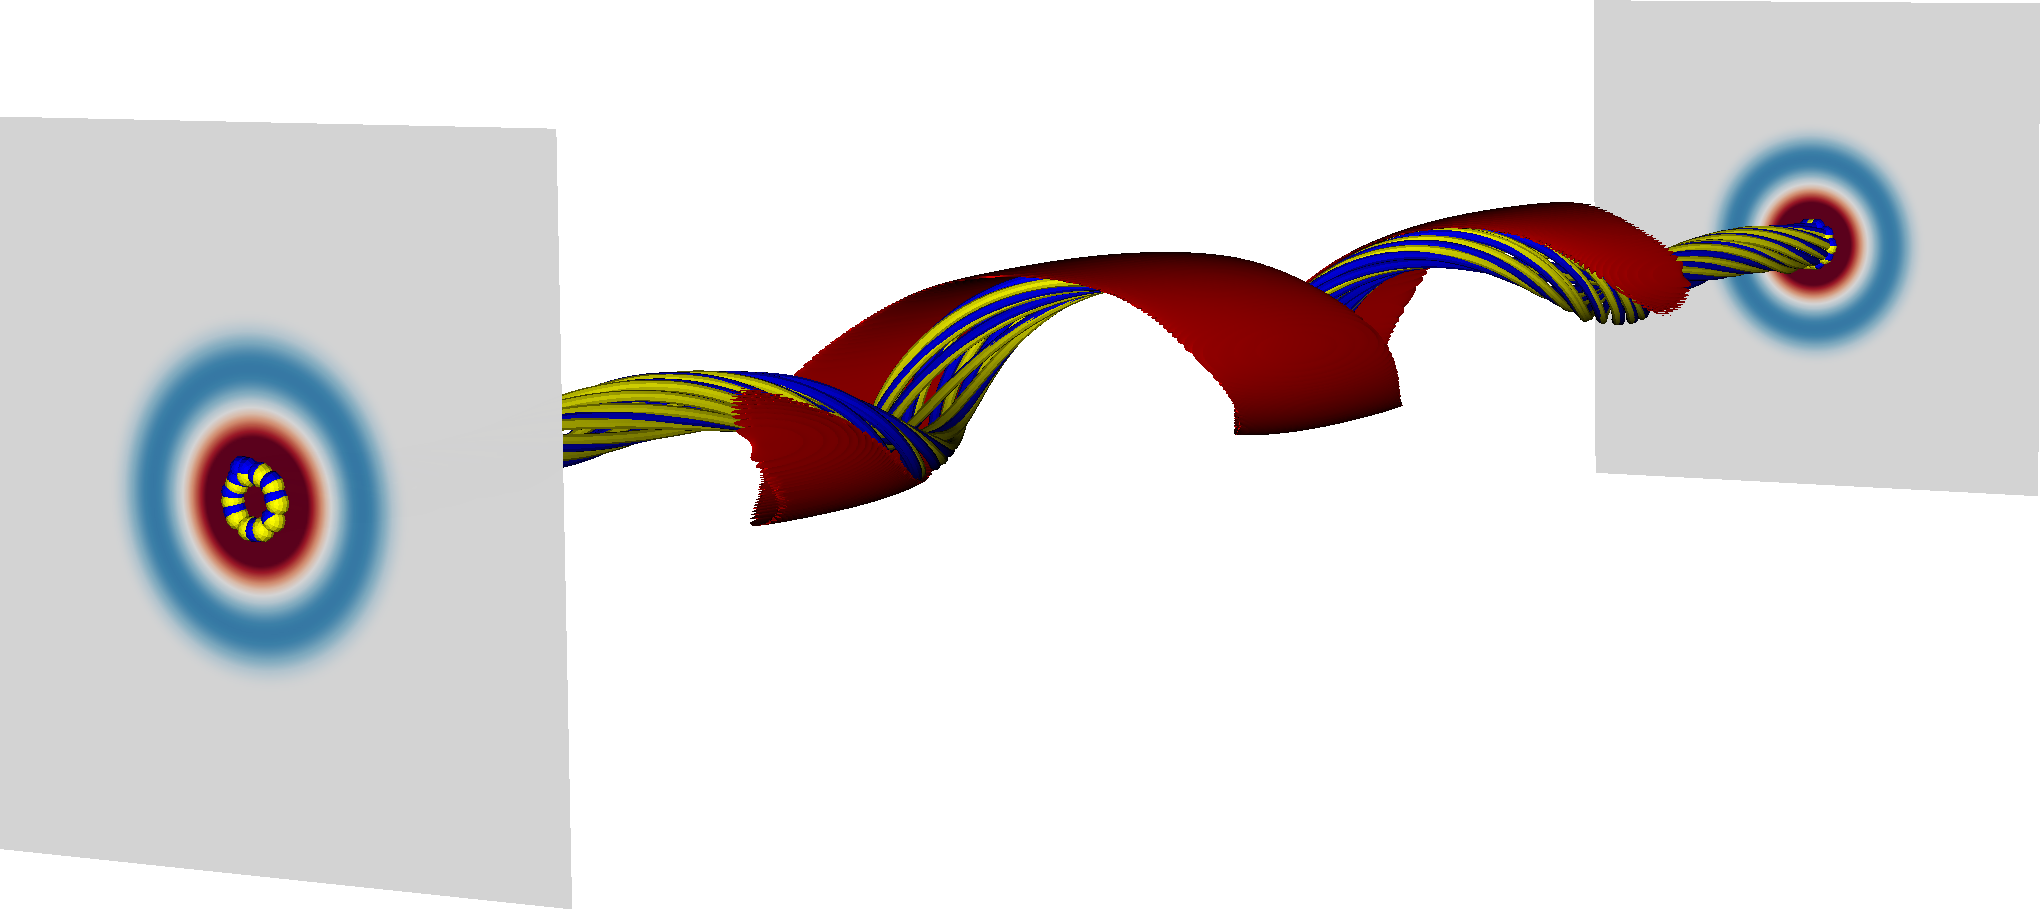
\includegraphics[width=\linewidth]{field_line_plots/cropped/v1e-4r5e-4.5-isotropic_0009_cropped.png}
      \caption{$t=45$}
      \label{fig:field_lines_0009}
    \end{subfigure}
    \begin{subfigure}{0.49\textwidth}
      \includegraphics[width=\linewidth]{field_line_plots/cropped/v1e-4r5e-4.5-isotropic_0010_cropped.png}
      \caption{$t=50$}
      \label{fig:field_lines_0010}
    \end{subfigure}
\caption{\textit{The transition from linear to nonlinear instability in the isotropic case.} The yellow field lines start at $z=10$ and the blue field lines at $z=-10$. The isosurfaces are at $|\vec{\jmath}| = 4$. The slices are plots of $\alpha(r)$. The linear growth of the instability ends around $t=35$ and the inner field compresses into the outer field, creating a current sheet. Between $t=45$ and $50$ this current sheet enables reconnection between the two regions. The transition for the switching case is qualitatively similar. In all three plots, $\nu = 10^{-4}$ and $\eta = 5\times 10^{-4.5}$, respectively.}
\label{fig:reconnecting_field_lines}%
\end{figure}

Initially, the instability occurs in the inner region of twist, $r<0.5$, where the magnetic field kinks helically. This section of the magnetic field compresses into the outer region, creating a current sheet along the length of the tube as shown in Figure~\ref{fig:field_lines_0009}. As the field continues to be compressed, it provides a magnetic pressure force that stalls the linear growth. The greater kinetic energy in the switching case leads to greater compression and thus a larger (though not notably stronger) current sheet. After this point, the growth of the kink instability is no longer in the linear phase.

During the transition from the linear to the nonlinear phase, field lines in the current sheet between the regions of inner and outer twist start to reconnect (Figures~\ref{fig:reconnection-field-lines}). This happens sooner in the switching case, due to the larger compression.

\subsection{Nonlinear phase}

\begin{figure}[t]
    \centering
    \begin{subfigure}[t]{0.49\textwidth}
      \centering
      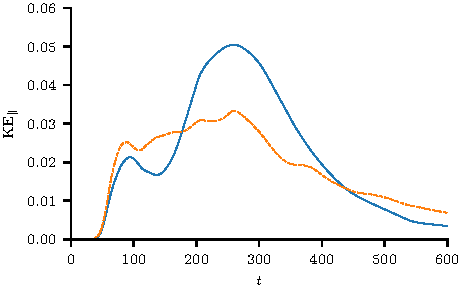
\includegraphics[width=\linewidth]{parallel_kinetic_energy_over_time.pdf}
      \caption{Parallel kinetic energy}
      \label{fig:parallel_kinetic_energy_over_time}
    \end{subfigure}%
    \begin{subfigure}[t]{0.49\textwidth}
      \centering
      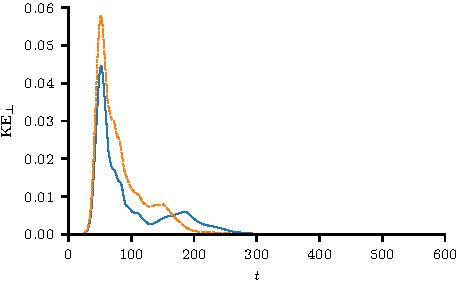
\includegraphics[width=\linewidth]{perp_kinetic_energy_over_time.pdf}
      \caption{Perpendicular kinetic energy}
      \label{fig:perp_kinetic_energy_over_time}
    \end{subfigure}
    \begin{subfigure}[t]{0.49\textwidth}
      \centering
      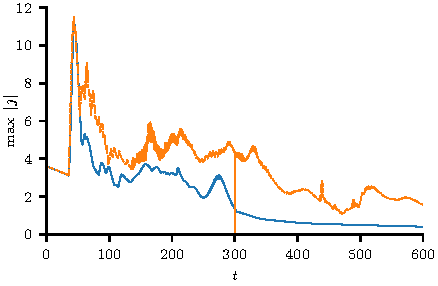
\includegraphics[width=\linewidth]{current_density_over_time.pdf}
      \caption{Maximum current density}
      \label{fig:current_density_over_time}
    \end{subfigure}
    \begin{subfigure}[t]{0.49\textwidth}
      \centering
      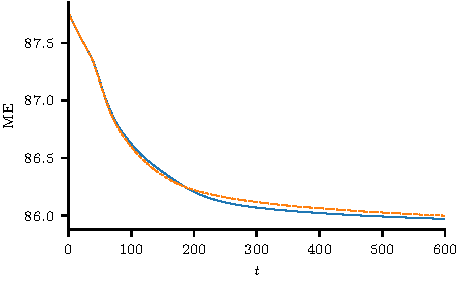
\includegraphics[width=\linewidth]{magnetic_energy_density_over_time.pdf}
      \caption{Magnetic energy}
      \label{fig:magnetic_energy_density_over_time}
    \end{subfigure}
    \caption{\textit{Energy components and current as functions of time.} Both isotropic (blue, solid) and switching (orange, dashed) viscosity models are shown, with diffusion parameters $\nu = 10^{-4}$ and $\eta = 5\times 10^{-4.5}$.}
    \label{fig:energies}
\end{figure}

Although the choice of viscosity model has a small effect on the
linear phase of the kink instability, it does play an important role
in the development of the nonlinear phase. By examining the kinetic
energies (KEs) in Figures~\ref{fig:energies}(a) and (b), a pattern
emerges in both cases that has similarities with the nonlinear
  behaviour of kink instabilities described in Hood et
al.~\cite{hoodCoronalHeatingMagnetic2009}. Shortly after the linear
phase, at $t\approx50$, the KEs for both viscosity models
exhibits a sharp rise, with the KEs associated with the switching
model attaining higher amplitudes. At the same time, a sharp rise is
also found in the maximum current as seen in
Figure~\ref{fig:energies}(c) and, leading on from this spike, the
current magnitudes associated with the switching model are larger than
those associated with the isotropic model. Returning to the KEs, the
energies associated with the switching model are greater until
$t\approx175$, after which, in \emph{only} the isotropic case, 
a clear secondary spike in perpendicular kinetic energy is found, along with a large
increase in parallel kinetic energy, much greater than the corresponding energy
found in the switching case. It is difficult to detect this new phase
in the maximum current (Figure~\ref{fig:energies}(c)), but it is found
in other quantities related to magnetic reconnection. 

\begin{figure}[t]
    \centering
    \begin{subfigure}[t]{0.5\textwidth}
      \centering
      \includegraphics[width=\linewidth]{max_parallel_electric_field.pdf}
      \caption{Parallel electric field}
      \label{fig:max_parallel_electric_field}
    \end{subfigure}%
    ~
    \begin{subfigure}[t]{0.5\textwidth}
      \centering
      \includegraphics[width=\linewidth]{mean_difference_in_connectivity.pdf}
      \caption{Difference in connectivity}
      \label{fig:mean_difference_in_connectivity}
    \end{subfigure}
    \caption{\textit{Reconnection rates.} The maximum integrated parallel electric field and mean difference in connectivity are plotting for the isotropic (blue dot \& solid line) and switching (orange cross \& dashed line) cases with $\nu = 10^{-4}$ and $\eta = 5\times 10^{-4.5}$. The difference in time between each data point is $5$ Alfv\'en times.}
    \label{fig:reconnection-rates}
\end{figure}

Figure~\ref{fig:reconnection-rates} displays the time series of the maximum integrated parallel electric field and the mean difference in connectivity, for both viscosity models. Both of the time series in Figure~\ref{fig:reconnection-rates} display similar trends to those found in the perpendicular kinetic energy plot, Figure~\ref{fig:energies}(a). For both isotropic and anisotropic viscosity there appears to be two major peaks in the reconnection measures that align with peaks in the perpendicular kinetic energy. This is much more obvious in the isotropic case. Both viscosity models allow for two phases of reconnection but the time at which they occur is significantly modified by the form of viscosity chosen. It is, therefore, clear that the form of viscosity is having a significant effect on the nonlinear evolution of the kink instability, both on the flow dynamics and the reconnection of the magnetic field. The following section presents, in more detail, the two important phases indicated by the isotropic time series, and how the results differ in the switching case.

\subsection{First phase: $t\approx65$--$100$}

\begin{figure}[t]
  \centering
  \begin{subfigure}[t]{0.32\textwidth}
    \centering
    \includegraphics[width=\linewidth]{slices/final_isotropic_current_density_0013.pdf}
    \caption{iso; $t=65$}
    \label{fig:final_isotropic_current_density_0013}
  \end{subfigure}
  \hfill
  \begin{subfigure}[t]{0.32\textwidth}
    \centering
    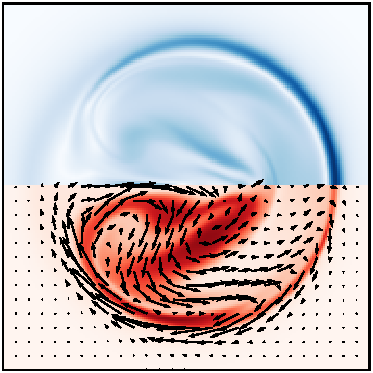
\includegraphics[width=\linewidth]{slices/final_isotropic_current_density_0015.pdf}
    \caption{iso; $t=75$}
    \label{fig:final_isotropic_current_density_0015}
  \end{subfigure}
  \hfill
  \begin{subfigure}[t]{0.32\textwidth}
    \centering
    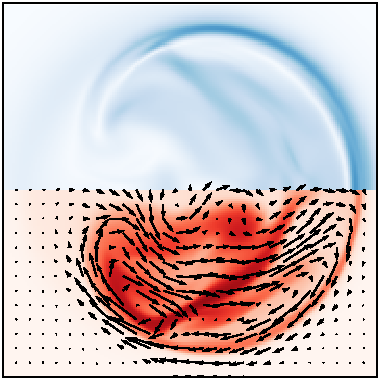
\includegraphics[width=\linewidth]{slices/final_isotropic_current_density_0020.pdf}
    \caption{iso; $t=100$}
    \label{fig:final_isotropic_current_density_0020}
  \end{subfigure}
  \hfill
  \begin{subfigure}[t]{0.32\textwidth}
    \centering
    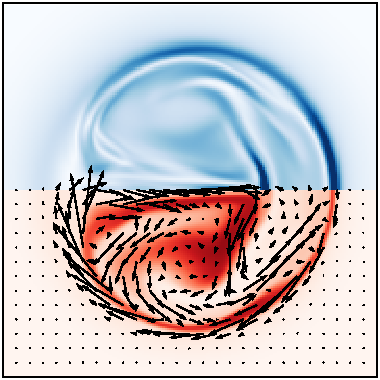
\includegraphics[width=\linewidth]{slices/final_switching_current_density_0013.pdf}
    \caption{swi; $t=65$}
    \label{fig:final_switching_current_density_0013}
  \end{subfigure}
  \hfill
  \begin{subfigure}[t]{0.32\textwidth}
    \centering
    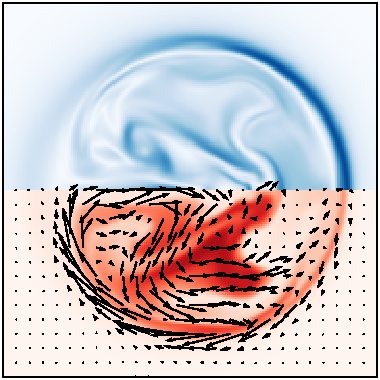
\includegraphics[width=\linewidth]{slices/final_switching_current_density_0015.pdf}
    \caption{swi; $t=75$}
    \label{fig:final_switching_current_density_0015}
  \end{subfigure}
  \hfill
  \begin{subfigure}[t]{0.32\textwidth}
    \centering
    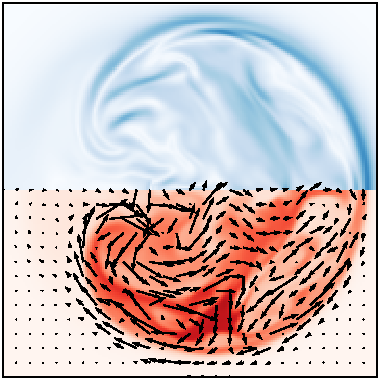
\includegraphics[width=\linewidth]{slices/final_switching_current_density_0020.pdf}
    \caption{swi; $t=100$}
    \label{fig:final_switching_current_density_0020}
  \end{subfigure}
  \caption{\textit{The difference in the evolution of current density,
      temperature and velocity structures between the isotropic
        and the switching viscosity cases}. Slices at $z=0$ of
    current density (top of each figure; blue is $|\vec{\jmath}| =
    3.5$, white is $|\vec{\jmath}| = 0$) and temperature (bottom of
    each figure; red is $T = 5\times10^{-2}$, white is
    $T=1.15\times10^{-5}$), overlaid with fluid flow. The halves shown are identical to their unseen counterparts, for both temperature and current density. That is, the simulation is vertically symmetrical at these times. The profile is cropped to
    $x=\pm1,\ y=\pm1$. The top three panels show the
    isotropic case and the bottom three panels show the switching case.}
  \label{fig:turning-point}
\end{figure}

At $t=65$, an intense current structure appears near the centre of the
tube for both viscosity models, although it is much stronger in the
switching case as illustrated in Figure~\ref{fig:turning-point}. Since the viscous damping associated with parallel viscosity is much less than that of isotropic viscosity, the flows in the switching case are stronger than those in the isotropic case (Figures~\ref{fig:energies}(a) and (b)). The faster flows drive stronger reconnection in the central current structure (see Figure~\ref{fig:reconnection-rates}) and the interaction of these processes leads to stronger outflows and finer-scale structures in the switching model case compared with the isotropic model case. Evidence of this behaviour can be seen by comparing the current and flow structures in Figure~\ref{fig:turning-point}. The effects of this phase can also be seen in the magnetic energy evolution, shown in Figure~\ref{fig:energies}(d). Between times $t=100$ and $125$, due to stronger reconnection in the switching case, the magnetic field relaxes marginally faster than that of the isotropic case, before the secondary instability begins in the isotropic case around $t=125$.

\begin{figure}[t]
  \centering
  \begin{subfigure}[t]{0.32\textwidth}
    \centering
    \includegraphics[width=\linewidth]{slices/final_isotropic_current_density_0025.pdf}
    \caption{iso; $t=125$}
    \label{fig:final_isotropic_current_density_0025}
  \end{subfigure}
  \hfill
  \begin{subfigure}[t]{0.32\textwidth}
    \centering
    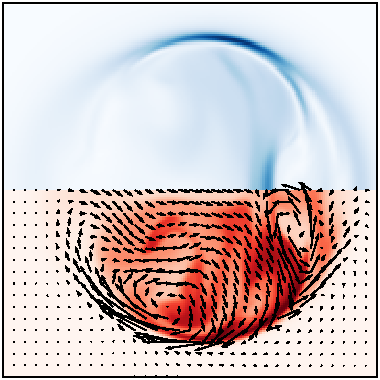
\includegraphics[width=\linewidth]{slices/final_isotropic_current_density_0030.pdf}
    \caption{iso; $t=150$}
    \label{fig:final_isotropic_current_density_0030}
  \end{subfigure}
  \hfill
  \begin{subfigure}[t]{0.32\textwidth}
    \centering
    \includegraphics[width=\linewidth]{slices/final_isotropic_current_density_0035.pdf}
    \caption{iso; $t=175$}
    \label{fig:final_isotropic_current_density_0035}
  \end{subfigure}
  \hfill
  \begin{subfigure}[t]{0.32\textwidth}
    \centering
    \includegraphics[width=\linewidth]{slices/final_switching_current_density_0025.pdf}
    \caption{swi; $t=125$}
    \label{fig:final_switching_current_density_0025}
  \end{subfigure}
  \hfill
  \begin{subfigure}[t]{0.32\textwidth}
    \centering
    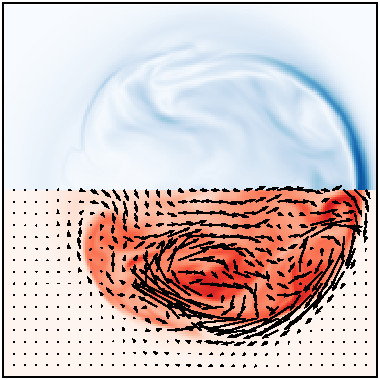
\includegraphics[width=\linewidth]{slices/final_switching_current_density_0030.pdf}
    \caption{swi; $t=150$}
    \label{fig:final_switching_current_density_0030}
  \end{subfigure}
  \hfill
  \begin{subfigure}[t]{0.32\textwidth}
    \centering
    \includegraphics[width=\linewidth]{slices/final_switching_current_density_0035.pdf}
    \caption{swi; $t=175$}
    \label{fig:final_switching_current_density_0035}
  \end{subfigure}
  \caption{\textit{The formation of a reconnection feedback loop in the isotropic and the switching viscosity cases.} Plotting parameters are identical to those of Figure~\ref{fig:turning-point}. The isotropic case shows two current sheets causing reconnection at the top and bottom of the tube, producing flows that sustains another central current sheet, which feeds back into the top and bottom sheets. The switching case instead shows one single main current sheet at the right hand side, along with numerous smaller current structures throughout the domain.}
  \label{fig:feedback-reconnection}
\end{figure}

\subsection{Second phase: $t\approx125$--$175$}
The contrast between fine-scale current and flow structures for the switching model, and the smoother, larger-scale structures of the isotropic model continues to be present at later times. Figure~\ref{fig:feedback-reconnection} shows the same data as Figure~\ref{fig:turning-point} but for the times $t=125$, $150$ and $175$. Looking at the slices for $t=125$, there is more fine-scale structure generated in the switching case compared to the isotropic case, as in the first phase described above. This second phase, however, marks the beginning of a significant change in behaviour in the isotropic model case. From Figure~\ref{fig:energies}, the parallel KE for the isotropic model exhibits a rapid and large increase in kinetic energy, characteristic of a secondary instability. To a lesser extent, there is also growth in the perpendicular KE, and the two reconnection measures for the isotropic model. In the second phase, these three measures increase to eventually become greater than their corresponding values for the switching model, around $t=175$. The significant difference in the behaviour between the two models are explored by first considering the slices in Figure~\ref{fig:feedback-reconnection}.

\begin{figure}[t]
  \centering
  \begin{subfigure}[b]{0.48\textwidth}
    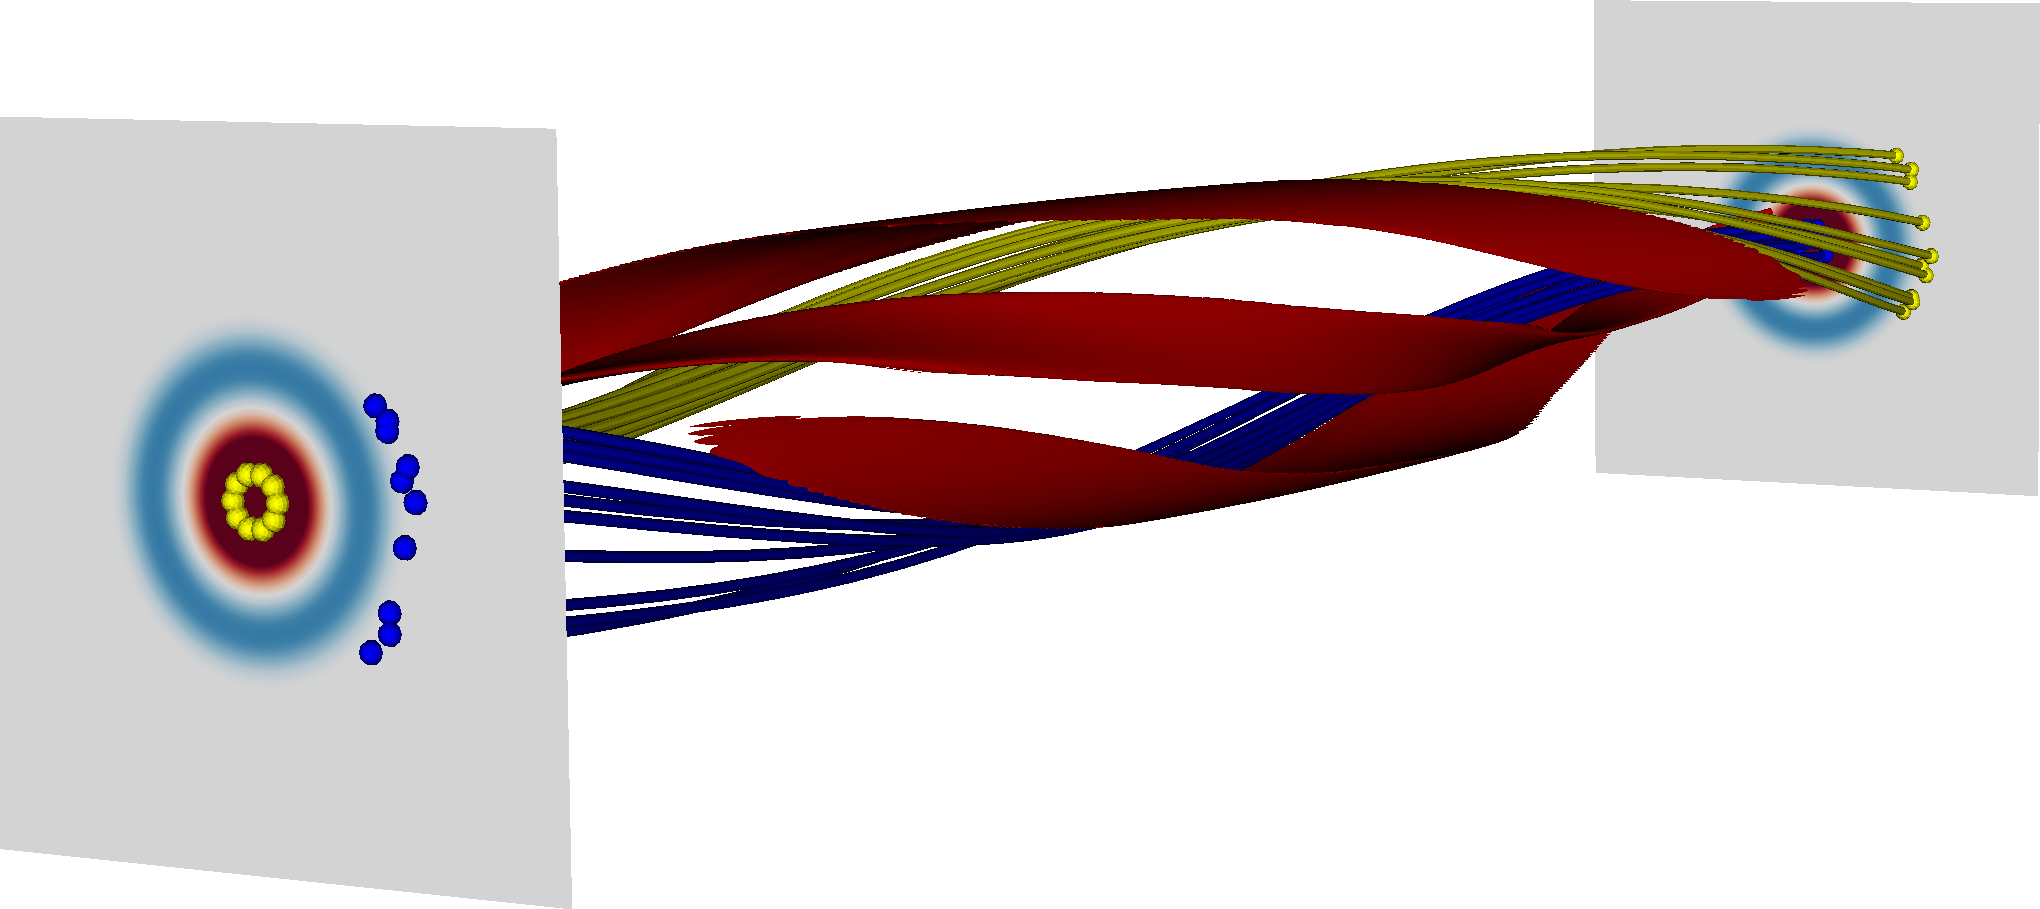
\includegraphics[width=\linewidth]{field_line_plots/cropped/v1e-4r5e-4.5-isotropic_0035_cropped.png}
    \caption{Isotropic}
    \label{fig:reconnection-field-lines-iso}
  \end{subfigure}
  \begin{subfigure}[b]{0.48\textwidth}
    \includegraphics[width=\linewidth]{field_line_plots/cropped/v1e-4r5e-4.5-switching_0035_cropped.png}
    \caption{Switching}
    \label{fig:reconnection-field-lines-swi}
  \end{subfigure}
  \caption{\textit{The difference in 3D current structures at $t=175$.} Isosurfaces are at $|\vec{\jmath}| = 1.5$.}
\label{fig:reconnection-field-lines}
\end{figure}

At $t=125$ (panels (a) and (d) of Figure~\ref{fig:feedback-reconnection}), the difference in behaviour
between the models is similar to the first phase but some new features
appear. The KE in the isotropic model begins to increase and, as
mentioned before, appears to signify a secondary instability. In
Figure~\ref{fig:feedback-reconnection}(a), two new current sheets have
formed at the top and bottom of the tube. A three-dimensional (3D)
visualisation of these current sheets is shown in
Figure~\ref{fig:reconnection-field-lines-iso}. The outflow from the
reconnection occurring within these current sheets then creates two
new symmetric vortices on the right hand side of the tube, advecting
the field into the centre of the tube. This behaviour can be seen
clearly in Figure~\ref{fig:feedback-reconnection}(b) where vortex
motion compresses the magnetic field and forms a central region of
enhanced current density. Later, as seen at $t=175$ in Figure~\ref{fig:feedback-reconnection}(c), the central current region becomes stronger due to continued compression and reconnection ensues, becoming stronger than the switching model case (see Figure~\ref{fig:reconnection-rates}). The outflows from this current region then feed into the vortical motions that drive the compression. In this way, a feedback loop is set up, and the reconnection within the current structure continuously drives the flow, resulting in an instability. This kind of interaction between multiple current sheets is also seen in~\cite{hoodCoronalHeatingMagnetic2009}. Due to this secondary instability, magnetic relaxation now becomes faster for the isotropic case. The magnetic energy for this case now dips below that of the switching case, as shown in Figure~\ref{fig:energies}(d).

During this phase, the kinetic energy in the switching model case also increases but to a much smaller extent compared to the isotropic model case. Although the current densities in Figures~\ref{fig:feedback-reconnection}(d) to (f) again exhibit finer-scale structure compared to the isotropic case, the magnitude of the current density within the tube becomes weaker with a more uniform profile developing in time. The dominating current sheets are on the edge of the tube, as also indicated in Figure~\ref{fig:reconnection-field-lines-swi}.

\subsection{Late-time states}

\begin{figure}[t]
  \centering
  \begin{subfigure}[b]{0.48\textwidth}
    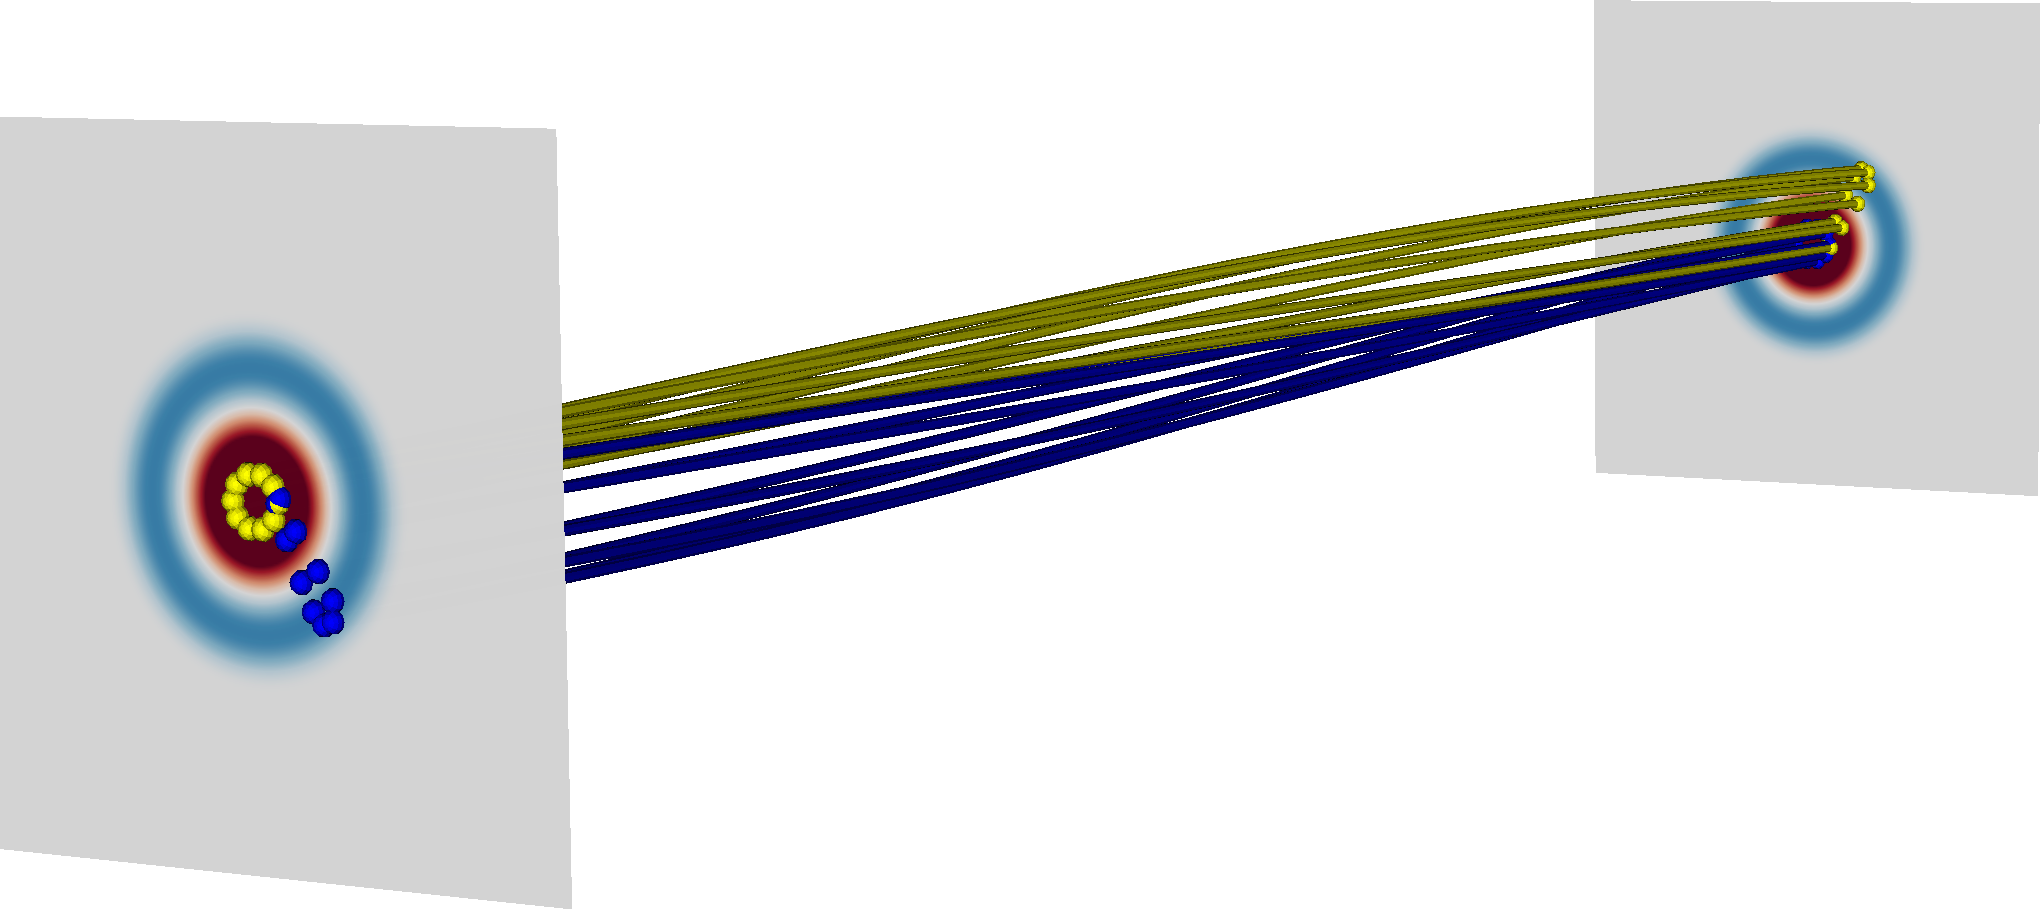
\includegraphics[width=\linewidth]{field_line_plots/cropped/v1e-4r5e-4.5-isotropic_0062_cropped.png}
    \caption{Isotropic}
  \end{subfigure}
  \begin{subfigure}[b]{0.48\textwidth}
    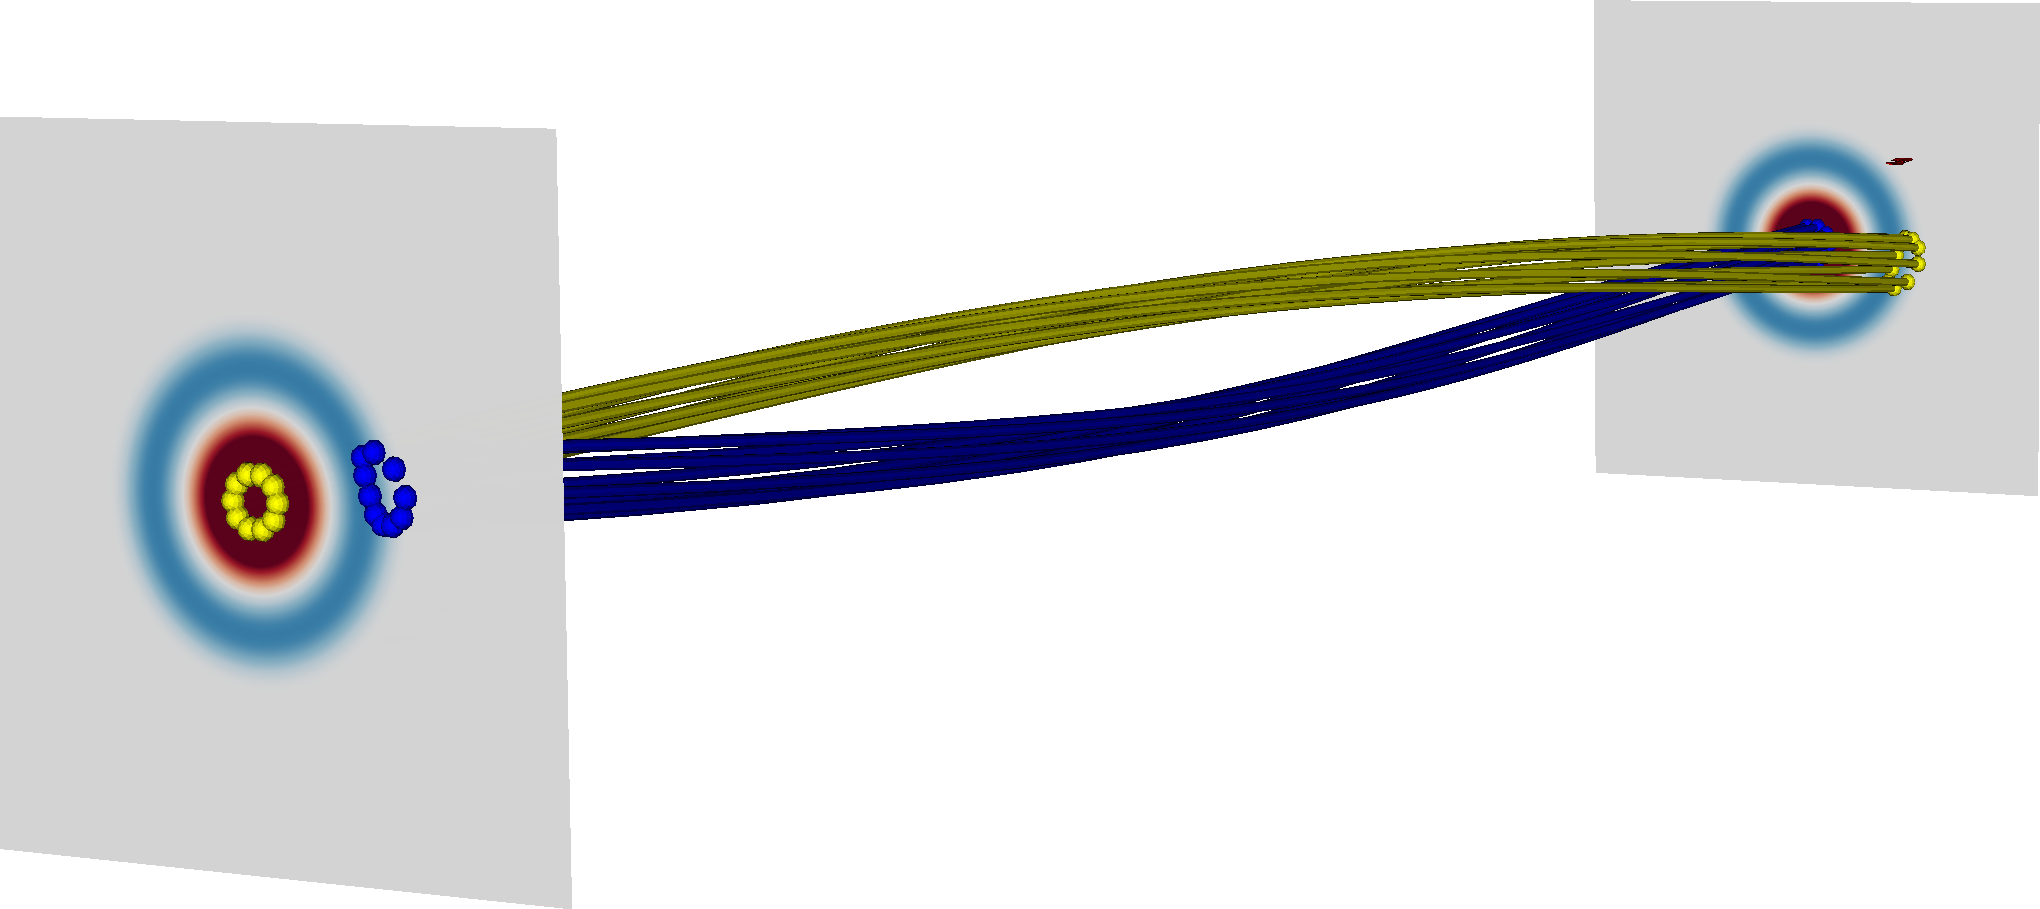
\includegraphics[width=\linewidth]{field_line_plots/cropped/v1e-4r5e-4.5-switching_0059_cropped.png}
    \caption{Switching}
  \end{subfigure}
  \caption{\textit{Late-time magnetic field structures at $t=600$.}}
\label{fig:finale-field-lines}
\end{figure}

For both cases, the asymptotic relaxed magnetic field is a linear force-free field. The route to this asymptotic state, however, depends on the viscosity model used. At the late time of $t=600$, there remain clear differences in the field structure between the two models resulting from the different nonlinear evolutions, as can be seen in Figure~\ref{fig:finale-field-lines}. At $t=600$, the magnetic field in the isotropic case (Figure~\ref{fig:finale-field-lines}(a)) appears straighter, indicative of more efficient magnetic relaxation. Indeed, Figure~\ref{fig:energies}(d) shows that more energy has been extracted from the field in the isotropic case. At $t=600$, the current density and energies (see Figure~\ref{fig:energies}) are still non-zero, so further relaxation is expected. For coronal applications, however, these late times are not as important as the early phases, described above, when the initial and secondary instabilities develop.

\subsection{Viscous and Ohmic heating}

\begin{figure}[t]
    \centering
    \begin{subfigure}[t]{0.32\textwidth}
      \includegraphics[width=\textwidth]{ohmic_heating_over_time.pdf}
      \caption{Ohmic heating}
    \end{subfigure}
    \begin{subfigure}[t]{0.32\textwidth}
      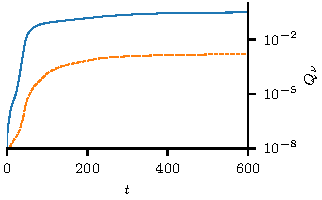
\includegraphics[width=\textwidth]{viscous_heating_over_time.pdf}
      \caption{Viscous heating}
    \end{subfigure}
    \begin{subfigure}[t]{0.32\textwidth}
      \includegraphics[width=\textwidth]{total_heating_over_time.pdf}
      \caption{Total heating}
    \end{subfigure}
    \caption{\textit{Heating rates as functions of time.} Plots are shown for isotropic (blue, solid) and switching (orange, dashed) viscosity, with diffusion parameters $\nu = 10^{-4}$ and $\eta = 5\times 10^{-4.5}$. Ohmic heating dominates isotropic viscous heating by an order of magnitude, and switching viscosity by four orders. Isotropic viscosity generates a factor of around $10^{3}$ more heat that switching viscosity. Even though more Ohmic heat is generated in the switching case, it does not compensate for the much weaker viscous heating.}
    \label{fig:heating}
\end{figure}

Over the lifetime of the entire instability the switching model allows for the generation of more Ohmic heating (Figure~\ref{fig:heating}(a)). This is despite the long, secondary phase of reconnection produced in the isotropic case. The greater heating in the switching case is due to two factors: the greater compression created by faster flows, creating stronger or larger current sheets and the more numerous current sheets created by more complex flows. However, isotropic viscous heating dominates that of the switching model by two orders of magnitude (Figure~\ref{fig:heating}(b)) ultimately leading to greater overall heating in the isotropic case (Figure~\ref{fig:heating}(c)). Physically, this is due to anisotropic viscosity only performing significant damping when velocity gradients align appropriately with the magnetic field (that is, when $(\ten{W} \vec{b}) \cdot \vec{b}$ is non-zero). 

Comparing Ohmic and viscous heating (Figures~\ref{fig:heating}(a) and (b)), Ohmic heating outperforms viscous heating in both cases, by an order of magnitude in the isotropic case and by three orders in the switching case. Even though similar values for the diffusion of the magnetic field $\eta$ and the velocity $\nu$ are used, during the kink instability the current sheets produced are much stronger than the gradients in velocity, hence the Ohmic heating dissipates more energy than the viscous heating.

Due to the relationship between $(\ten{W} \vec{b}) \cdot \vec{b}$ and $Q_{\nu}$ (equation~\eqref{eq:aniso_viscous_heating} with $s\approx 1$), the small magnitude of $Q_{\nu}$ in Figure~\ref{fig:heating}(b) implies that $(\ten{W} \vec{b}) \cdot \vec{b}$ is small everywhere. With the anisotropic viscous heating being heavily dependent on the magnetic field direction and since $(\ten{W} \vec{b}) \cdot \vec{b}$ is small everywhere in the kink simulation, it follows that the anisotropic viscous heating is always lower in magnitude compared to the isotropic viscous heating, which is not bound by the diection of the magnetic field.

\subsection{The effect of anisotropy on feedback reconnection}

I have described the nonlinear evolution of the kink instability for the cases of only isotropic viscosity and only anisotropic viscosity. When the viscosity is totally isotropic, the secondary instability is found, yet when the viscosity is totally anisotropic, the same instability is disrupted. To determine how anisotropic the viscosity must become before the secondary instability is disrupted, the degree of anisotropy can be fixed by artificially fixing the value of $s$ to some constant, instead of letting $s$ rely on the local field strength $|\vec{B}|$. It should be noted that the simulations in which $s$ is fixed are no longer physically realistic, but the results can be used to estimate the degree of anisotropy required in the viscosity to disrupt the secondary instability. Since the interpolation involves only $s^2$ instead of $s$, in practice the value of $s^2$ is fixed.

\begin{figure}[t]
  \centering
  \includegraphics[width=0.5\linewidth]{kinetic-energy-changing-s.pdf}
  \caption{\textit{Kinetic energy over time, varying the switching
        function $s^2$.} The grey lines are the two regular cases; switching, where $s^2 = 1$ (dashed), and isotropic (solid), where $s^2=0$. The coloured lines represent values of $s^2 = 0.5$ (blue, dotted), and $s^2 = 0.6$ (orange, dash-dotted). There is a clear critical value somewhere between $0.5$ and $0.6$, where the behaviour changes.}
  \label{fig:kinetic-energy-changing-s}
\end{figure}

By letting $s^2$ in equation~\eqref{eq:switching_model} take values between $0$ and $1$, it is found that there is not a smooth transition between the two extremes of behaviour. Instead, there is a critical value of $s^2$, between $0.5$ and $0.6$, below which (closer to isotropic) the resultant flows are simple enough to create and sustain feedback reconnection, and above which (closer to anisotropic) the flows are sufficiently complex to disrupt the secondary instability. This behaviour can be seen in how the kinetic energy time series changes with $s^2$ in Figure~\ref{fig:kinetic-energy-changing-s}.

\section{Parameter study}
\label{sec:results2}

In order to confirm that the results of Section~\ref{sec:results} are typical, and to further understand how they vary, two parameter studies are performed; one varying viscosity, keeping all other parameters constant; and one varying resistivity, again keeping all other parameters constant. 

In the first study the viscosity is varied as $\nu = 5 \times 10^{-n}$, where the index $n$ takes the values $4.75$, $4.5$, $4.25$, $4$ and $3.75$, while keeping resistivity constant at $\eta = 5\times10^{-4.5}$. This range of viscosities represents values that are typically used in simulations, with a lower bound above numerical diffusion and an upper bound below physically unrealistic values for the corona.

In the second study the resistivity is similarly varied as $\eta = 5 \times 10^{-m}$, where the index $m$ takes the values $4.75$, $4.5$, $4.25$, $4$, $3.75$, and $3.5$, while keeping the resistivity constant at $\nu = 5\times 10^{-4.5}$. Similar to the limits on viscosity, any lower resistivities become comparable to numerical diffusion. Higher resistivities diffuse the field so quickly that the instability does not have time to grow.

\subsection{Effect on the secondary instability varying diffusion parameters}
\label{sec:secondary_instability}

\begin{figure}[t]
    \centering
    \begin{subfigure}[t]{0.5\textwidth}
      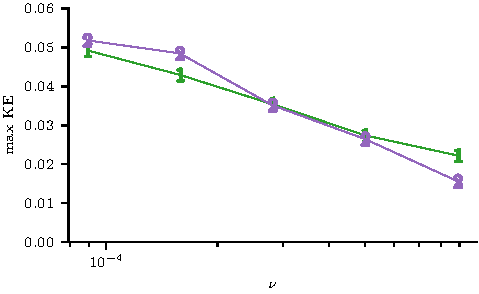
\includegraphics[width=\textwidth]{max_ke_split_inst_changing_viscosity.pdf}
      \caption{Varying viscosity; $\eta = 5\time 10^{-4.5}$}
    \end{subfigure}%
    ~
    \begin{subfigure}[t]{0.5\textwidth}
      \includegraphics[width=\textwidth]{max_ke_split_inst_changing_resistivity.pdf}
      \caption{Varying resistivity; $\nu = 5\time 10^{-4.5}$}
    \end{subfigure}
    \caption{\textit{Maximum kinetic energy corresponding to initial instability and secondary instability as functions of resistivity $\eta$ and viscosity $\nu$.} In both plots are shown the maximum kinetic energy produced by the initial instability (green, $1$-marker) and the maximum kinetic energy produced by the secondary instability (purple, $2$-marker). Only results using the isotropic viscosity are shown.}
    \label{fig:secondary_instability}
\end{figure}

Figure~\ref{fig:secondary_instability} shows the maximum kinetic energy produced by the two instabilities found in the isotropic case in Section~\ref{sec:results}. The maximum kinetic energy provides a useful measure of the efficacy of an instability, particularly when comparing the relative magnitudes of the initial and secondary instabilities. Since only the isotropic case reveals evidence of the secondary instability, results from the switching case are not shown.

Looking at Figure~\ref{fig:secondary_instability}(a), it is observed that increasing $\nu$ reduces the kinetic energy generated in both instabilities. For small values of $\nu$ the secondary instability causes more energy to be produced than the first, however as $\nu$ increases, this relationship reverses, with the initial instability causing more energy to be produced than the secondary one for large $\nu$. This reversal suggests that the greater kinetic energy produced by the initial instability for low values of $\nu$ is causing a stronger current sheet to form, enhancing reconnection, and producing a stronger secondary instability.

The effect of resistivity $\eta$ on the secondary instability is to suppress it entirely when $\eta$ is large. Since the secondary instability is driven by reconnection outflows, it is not surprising that there are values of $\eta$ for which the reconnection outflows do not feedback to produce the instability.

\subsection{Varying viscosity}

\label{sec:visc_param_study}

\subsubsection{Dependence of heating on viscosity}

\begin{figure}[t]
    \centering
    \begin{subfigure}[t]{0.32\textwidth}
      \includegraphics[width=\textwidth]{visc_heating_varying_viscosity.pdf}
      \caption{Viscous heating}
    \end{subfigure}%
    ~
    \begin{subfigure}[t]{0.32\textwidth}
      \includegraphics[width=\textwidth]{ohmic_heating_varying_viscosity.pdf}
      \caption{Ohmic heating}
    \end{subfigure}
    ~
    \begin{subfigure}[t]{0.32\textwidth}
      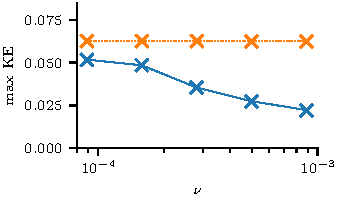
\includegraphics[width=\textwidth]{max_kinetic_changing_visc.pdf}
      \caption{Maximum kinetic energy}
    \end{subfigure}
    \caption{\textit{Anisotropic viscous heating, Ohmic heating, and maximum kinetic energy as functions of viscosity $\nu$.} Plots are shown using isotropic viscosity (blue, solid) and switching viscosity (orange, dashed) as functions of viscosity $\nu$ at the final time of $t=400$ for a fixed resistivity $\eta=5\times10^{-4.5}$, The anisotropic viscous heating has been multiplied by a factor of $10$. The maximum kinetic energy is calculated as the maximum value prior to $t=400$.}
    \label{fig:param_study_varying_viscosity}
\end{figure}

Figures~\ref{fig:param_study_varying_viscosity}(a) and~\ref{fig:param_study_varying_viscosity}(b) show the total heat generated by $t=400$ via viscous $Q_{\nu}$ and Ohmic $Q_{\eta}$ dissipation as $\nu$ is varied. It should be noted that, to allow the trend in the anisotropic viscous heating to be seen in the plot, it has been multiplied by a factor of $10$. Before discussing the apparent trends in the heating as $\nu$ is varied, it is useful to note that, just as in the typical case described previously, for the range of $\nu$ shown, isotropic viscous heating remains approximately two orders of magnitude greater than the anisotropic viscous heating, and the Ohmic heating is consistently higher when using anisotropic viscosity than when using isotropic.

Since viscous dissipation (equations~\eqref{eq:iso_viscous_heating} and~\eqref{eq:aniso_viscous_heating}) has a functional dependence on $\nu$ and Ohmic dissipation (equation~\eqref{eq:ohmic_heating}) does not, it could be naively assumed that variation in viscosity should present some trend in the viscous dissipation for both models and no trend in the Ohmic dissipation. The trends that are observed broadly adhere to this but, unexpectedly there appears some trend in the Ohmic heating when using isotropic viscosity.

When employing the switching model, the Ohmic heating appears to be independent of $\nu$, whereas when employing the isotropic model, there appears a small trend of decreased Ohmic heating with increased $\nu$. These trends can be explained by considering the effect of viscosity on compressive flows and current densities. During the kink instability, Ohmic heating, being proportional to the square of the local current density, is increased when an already sheared magnetic field is compressed by flows perpendicular to the field, increasing the local current density. Thus, as the speeds of perpendicular flows increase, so does the Ohmic heating. These perpendicular flows are effectively only damped by isotropic viscosity. Since the maximum kinetic energy (Figure~\ref{fig:param_study_varying_viscosity}(c)) decreases with $\nu$ in \emph{only} the isotropic case, and remains constant in the switching case, it is appropriate that the Ohmic heating decreases with $\nu$ in the isotropic case and is negligibly dependent on $\nu$ in the switching case.

If varying $\nu$ does not change the dynamics in the switching case, the functional dependence of $Q_{\nu}$ on $\nu$ (see equation~\eqref{eq:aniso_viscous_heating}) suggests an increase in anisotropic viscous heating with $\nu$ should be observed. Figure~\ref{fig:param_study_varying_viscosity}(a) reveals precisely this.

The relationship between the isotropic viscous heating at $\nu$ appears non-trivial. Given the decrease in maximum kinetic energy (Figure~\ref{fig:param_study_varying_viscosity}(a)) with $\nu$, it is expected the isotropic viscous heating should also decrease. However, this is not what is observed. Although there appears to be a slight decreasing trend in the isotropic viscous heating when $\nu$ is increased past $10^{-4}$, the left-most point is clearly an outlier. This suggests the secondary instability is having a significant and non-trivial effect on the heating. Indeed this is also suggested by the subtle change of gradient in the maximum kinetic energy on the left-hand side of the Figure~\ref{fig:param_study_varying_viscosity}(c). Due to this particular parameter study producing only five data points, these trends cannot be discussed with much confidence. A more detailed parameter study should be performed, investigating more values of $\nu$ within and beyond the range studied here.

\subsubsection{Dependence of linear growth rate on viscosity}
\label{sec:linear_growth_rate_varying_visc}

\begin{figure}[t]
    \centering
    \begin{subfigure}[t]{0.5\textwidth}
      \includegraphics[width=\textwidth]{growth_rate_varying_viscosity.pdf}
      \caption{Growth rate}
    \end{subfigure}%
    ~
    \begin{subfigure}[t]{0.5\textwidth}
      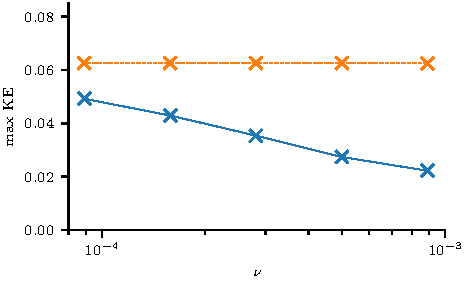
\includegraphics[width=\textwidth]{max_early_time_kinetic_changing_visc.pdf}
      \caption{Maximum early-time kinetic energy}
    \end{subfigure}
    \caption{\textit{Linear growth rate and maximum (in time) kinetic energy as
        functions of viscosity $\nu$ for a fixed
          resistivity of $\eta=5\times10^{-4.5}$.} Plots are shown using isotropic viscosity (blue, solid) and switching viscosity (orange, dashed) as functions of viscosity $\nu$. The maximum kinetic energies are calculated as the maximum values in time prior to $t=125$. This is to capture the behaviour of only the initial nonlinear evolution of the instability, neglecting any further instabilities like the secondary instability found in Section~\ref{sec:results}. Note, the maxima do not necessarily occur at the same time and this particular parameter study has been performed fixing $\nu$ at a slightly different value to the previous parameter studies.}
    \label{fig:growth_rate_varying_viscosity}
\end{figure}

For each value of $\eta$ the linear growth rate $\sigma$ of the onset of the kink instability is estimated by plotting the logarithm of the kinetic energy against time and measuring the gradient during the period of linear growth (as is done in Figure~\ref{fig:log_kinetic_energy_over_time}). Figure~\ref{fig:growth_rate_varying_viscosity}(a) plots these growth rates against $\eta$, and Figure~\ref{fig:growth_rate_varying_viscosity}(b) shows the maximum kinetic energy calculated as the maximum prior to $t=125$. For every $\eta$, this time is between the peaks of the kinetic energy corresponding to the first and secondary instabilities. Taking the maximum before this time allows us to capture only the behaviour of the initial instability, since this is the instability of interest in this section.

It can be seen from the relationship between the growth rate and $\nu$ for both viscosity models that isotropic viscosity appears to begin to suppress the kink instability, for larger $\nu$, while the switching viscosity does not (Figure~\ref{fig:growth_rate_varying_viscosity}(a)). This is also apparent from the relationship between the maximum kinetic energy and $\nu$ for both models (Figure~\ref{fig:growth_rate_varying_viscosity}(b)). This difference between the viscosity models results from the anisotropic viscosity being so weak that the dynamics of the initial onset of the kink instability are not significantly affected by a significant increase in $\nu$.

\subsection{Varying resistivity}

\subsubsection{Dependence of heating on resistivity}

\begin{figure}[t]
    \centering
    \begin{subfigure}[t]{0.5\textwidth}
      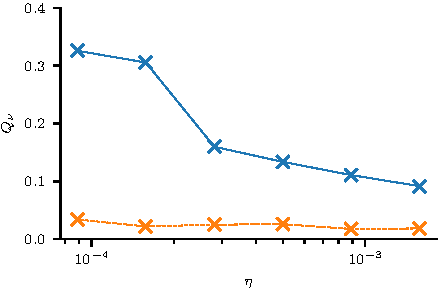
\includegraphics[width=\textwidth]{visc_heating_varying_resistivity.pdf}
      \caption{Viscous heating}
    \end{subfigure}%
    ~
    \begin{subfigure}[t]{0.5\textwidth}
      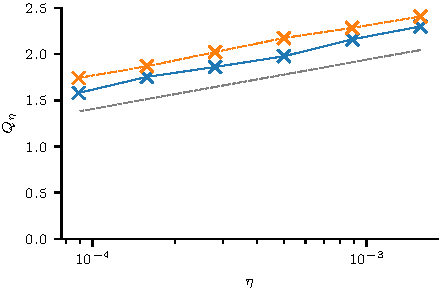
\includegraphics[width=\textwidth]{ohmic_heating_varying_resistivity.pdf}
      \caption{Ohmic heating}
    \end{subfigure}
    \caption{\textit{Anisotropic viscous, and Ohmic heating as functions of resistivity $\eta$ for a fixed value of viscosity $\nu=5\times10^{-4.5}$.} Plots are shown using isotropic viscosity (blue, solid) and switching viscosity (orange, dashed) as functions of resistivity $\eta$ at the final time of $t=400$. The anisotropic viscous heating has been multiplied by a factor of $10$. Overlaid on Figure (b) is the scaling $\log_{10}(\eta^{1/2})$.}
    \label{fig:param_study_varying_resistivity}
\end{figure}

Figure~\ref{fig:param_study_varying_resistivity}(a) and~\ref{fig:param_study_varying_resistivity}(b) show the total heating generated by $t=400$ via viscous $Q_{\nu}$ and Ohmic $Q_{\eta}$ dissipation as the strength of resistivity $\eta$ is varied. Just as in Section~\ref{sec:visc_param_study}, the anisotropic viscous heating is multiplied by $10$. Again, it is useful to note that, across the entire range of $\eta$ studied here, the isotropic viscous heating remains approximately two orders of magnitude greater than the anisotropic viscous heating and the Ohmic heating produced when using switching viscosity is consistently higher than that produced when using isotropic viscosity. This aligns with the results when varying viscosity, as discussed above.

As in the parameter study varying $\nu$, a non-trivial relationship appears between the viscous heating for both models and $\eta$ (Figure~\ref{fig:param_study_varying_resistivity}(a)). The isotropic viscous heating reveals an decreasing trend over all values of $\eta$ studies here, however there is a clear jump in heating between approximately $10^{-3.9}$ and $10^{-3.7}$. Given that these are the values of $\eta$ where there is strong influence of the secondary instability on the kinetic energy output (see Section~\ref{sec:secondary_instability}), these results suggest it is the kinetic energy produced by the secondary instability that is being damped at low values of $\eta$.

Just as in the parameter study varying $\nu$, the anisotropic viscosity shows very little variability with $\eta$ (Figure~\ref{fig:param_study_varying_resistivity}(a)), even with the heating multiplied by a factor of $10$ for plotting. Despite the dynamics significantly changing with $\eta$, the effect of the anisotropic viscosity is so small that very little change in the heating is observed.

Ohmic heating is observed to increase with increasing $\eta$ (Figure~\ref{fig:param_study_varying_resistivity}(b)). This is to be expected given the functional dependence of $Q_{\eta}$ on $\eta$, however the actual scaling is not linear in $\eta$, as might be predicted from equation~\eqref{eq:ohmic_heating}. Rather, $Q_{\nu}$ varies linearly with $\log_{10}(\eta^{1/2})$ for the range of $\eta$ studied here. Without a more comprehensive parameter study covering more values of $\eta$, it is difficult to reason why the scaling takes this form. However, what is certain is that the use of anisotropic viscosity is consistently enhancing Ohmic heating across the range of $\eta$ studied here. This is due to the kink instability producing more kinetic energy in the switching case, which better compresses the magnetic field, creating stronger current sheets and thus enhancing Ohmic heating.

\subsubsection{Dependence of linear growth rate on resistivity}

\begin{figure}[t]
    \centering
    \begin{subfigure}[t]{0.5\textwidth}
      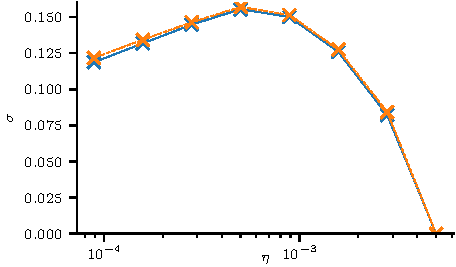
\includegraphics[width=\textwidth]{growth_rate_varying_resistivity.pdf}
      \caption{Growth rate}
    \end{subfigure}%
    ~
    \begin{subfigure}[t]{0.5\textwidth}
      \includegraphics[width=\textwidth]{max_kinetic_changing_resist.pdf}
      \caption{Maximum early-time kinetic energy}
    \end{subfigure}
    \caption{\textit{Linear growth rate and maximum (in time) kinetic energy as
        functions of resistivity $\eta$ for a fixed
          viscosity of $\nu=10^{-4}$.} \textbf{(a)} Growth rate and \textbf{(b)} maximum kinetic energy, generated by isotropic viscosity (blue, solid) and switching viscosity (orange, dashed) as functions of resistivity $\eta$. The maximum kinetic energies are calculated as the maximum values in time prior to $t=125$. This is to capture the behaviour of only the initial nonlinear evolution of the instability, neglecting any further instabilities like the secondary instability found in Section~\ref{sec:results}. Note, the maxima do not necessarily occur at the same time and this particular parameter study has been performed fixing $\nu$ at a slightly different value to the previous parameter studies.}
    \label{fig:growth_rate_varying_resistivity}
\end{figure}

As is done in Section~\ref{sec:linear_growth_rate_varying_visc}, the linear growth rates are measured for each value of $\eta$. These and the maximum early time ($t<125$) kinetic energy are shown in Figure~\ref{fig:growth_rate_varying_resistivity}. The plots show that the use of the switching model seems to consistently amplify the growth of the kink instability, shown both in the growth rate and in the kinetic energy. Beyond this, the two models of viscosity show similar trends with $\eta$.

Both plots in Figure \ref{fig:growth_rate_varying_resistivity} show that the kink instability is strongly inhibited for values of $\eta$ greater than approximately $10^{-2.5}$. This can be explained by the initial diffusion of the magnetic field being so fast-acting for large values of $\eta$ that the instability is totally suppressed. The increased suppression of the instability with strength of Ohmic diffusion can be seen in both plots as $\eta$ increases past $10^{-3}$.

\section{Discussion}

\label{sec:discussion}

Although there can be much variability in the nonlinear behaviour of the kink instability, these results reveal an important general finding. At the beginning of the nonlinear phase, anisotropic (parallel) viscosity allows for the development of smaller length scales (both flows and current sheets), compared to isotropic viscosity, leading to more efficient reconnection and faster magnetic relaxation, at least initially. As has been described in detail, isotropic viscosity can produce other effects later. However, for coronal applications, it is the initial nonlinear phase of the instability that is likely to be of most interest since, in reality, a coronal loop will interact with others on a longer time scale, thus affecting the nonlinear evolution. Since anisotropic viscosity is a more realistic model for viscosity in the corona, these results will be useful in the interpretation of observations of coronal loops that are kink unstable.

Additionally, the results of the parameter study reveal a potential scaling between Ohmic heating and resistivity. Extrapolating this to smaller values of $\eta$ than were investigated suggests that viscous heating will outperform Ohmic heating when $\eta\approx10{-7}$, a value greater than even generous estiates of anomolous resistivity of $\eta \approx 10^{-8}$. While there is no guarantee that the observed scaling will continue down to realistic resistivities, this finding does add to the body of evidence which argues that viscous heating is the dominant heating mechanism in the solar corona~\cite{craigAnisotropicViscousDissipation2009a,craigViscousDissipation3D2013}. 

\section{Conclusion}

\label{sec:conclusions}

This chapter details the linear and nonlinear development of the MHD kink
instability with two different viscosity models. The first is
isotropic (Newtonian) viscosity, which is the most commonly used
viscosity model in coronal loop studies. The second is anisotropic viscosity, representing the strong-field limit of Bragkinskii viscosity with a preferred direction parallel to the magnetic field. The implementation of anisotropic viscosity is via the von Mises switching model~\cite{mactaggartBraginskiiMagnetohydrodynamicsArbitrary2017}.

By considering particular (low) values of the viscosity and resistivity, it is found that the effect of the different viscosity models on the linear onset of the kink instability is marginal. The significant differences appear in the nonlinear phase. Two main phases of evolution can be identified which highlight the differences between the effects of the two viscosity models. The anisotropic (switching) case produces more kinetic energy at the onset of the nonlinear phase of the instability---the first phase. It also produces flows and current sheets with smaller length scales compared to the isotropic case and this allows the magnetic field to relax faster due to more efficient reconnection. 

In the second phase, the isotropic case exhibits a secondary instability, which is not found in the anisotropic case. This new instability leads to enhanced reconnection and faster magnetic relaxation, compared to the anisotropic case.  The simulations are run for $600$ Alfv\'en times (a long time period for coronal applications) and the behaviour of the second phase continues for all of this time.

A series of parameter studies was also run, where the strengths of viscosity and resistivity were varied. The qualitative results of the two phases of the detailed investigation hold true over a range of viscosities and resistivities, including the existence of the secondary instability. Notably, over all parameters studied, viscous heating is consistently overestimated by the isotropic model, and Ohmic heating is consistently enhanced by use of the switching model.
